\chapter{Wichtige Erläuterungen, Begriffsdefinitionen}\label{chap:Wichtige Erläuterungen, Begriffsdefinitionen}
\section{Remanenz}\label{sec:Remanenz}

Der Begriff \glqq Remanenz\grqq{} beschreibt die Eigenschaft, ob ein Datenpunkt über einen Neustart der CPU hinweg, auch bei Spannungsausfall, unverändert bleibt. Ist die Eigenschaft im globalen oder Instanz-Datenbaustein nicht aktiviert, werden bei CPU-Neustart dementsprechend für die betroffenen Variablen die parametrierten Startwerte als Aktualwerte geladen.

\clearpage

\section{Optimierte Bausteine}\label{sec:Optimierte Bausteine}

Dieses Kapitel und seine Unterkapitel sind aus dem Programmierleitfaden für S7-1200/S7-1500 übernommen \cite[13]{Siemens:SafetyS7_1200-1500}. Falls Verweise auf andere Kapitel aufgeführt und diese unterstrichen sind, beziehen sich die Verweise auf das entsprechende Kapitel im Leitfaden und nicht auf andere Kapitel in diesem Dokument.
S7-1200/1500 Steuerungen besitzen eine optimierte Datenablage. In optimierten Bausteinen sind alle Variablen gemäß ihres Datentyps automatisch sortiert. Durch die Sortierung wird sichergestellt, dass Datenlücken zwischen den Variablen auf ein Minimum reduziert werden und die Variablen für den Prozessor zugriffsoptimiert abgelegt sind.  
Nicht optimierte Bausteine sind in S7-1200/1500 Steuerungen nur aus Kompatibilitätsgründen vorhanden. 

\subsection{Vorteile}\label{subsec:Vorteile}

\begin{itemize}
    \item Der Zugriff erfolgt immer schnellstmöglich, da die Dateiablage vom System optimiert wird und unabhängig von der Deklaration ist.
    \item Keine Gefahr von Inkonsistenzen durch fehlerhafte, absolute Zugriffe, da generell symbolisch zugegriffen wird.
    \item Deklarationsänderungen führen nicht zu Zugriffsfehlern, da z.B. HMI-Zugriffe symbolisch erfolgen. 
    \item Einzelne Variablen können gezielt als remanent definiert werden.
    \item Keine Einstellungen im Instanzdatenbaustein notwendig. Es wird alles im zugeordneten FB eingestellt (z.B. Remanenz).
    \item Speicherreserven im Datenbaustein ermöglichen das Ändern ohne Verlust der Aktual Werte (siehe Kapitel 6.2.11 \textbf{"todo!"} Laden ohne Reinitialisierung).
\end{itemize}


\subsection{Nachteile}\label{subsec:Nachteile}
\textbf{ACHTUNG: Dieses Kapitel ist eine Ergänzung von Daniel Klein-Günnewick!}\par
\noindent Falls das SPS-Programm im TIA-Portal erstellt wird und die Visualisierung in einem externen System (z.B. WinCC V7.4) realisiert werden soll und gleichzeitig optimierter Zugriff eingestellt wurde, ist es nicht mehr möglich mit Strukturtypen auf die Steuerungsdaten zu schauen. In diesem Fall ist nur noch der Zugriff auf die Daten der SPS mit der Engineering-Funktion „Laden aus AS“  möglich. Um weiterhin strukturell auf Variablen zugreifen zu können, muss mit Bildfenstertechnik und Präfixen in den entsprechenden Systemen, z.B. WinCC V7.4 SP1, gearbeitet werden.
\clearpage

\subsection{S7-1200: Aufbau von optimierten Bausteinen}\label{subsec:S7-1200: Aufbau von optimierten Bausteinen}
\begin{figure}[!ht]
    \centering
    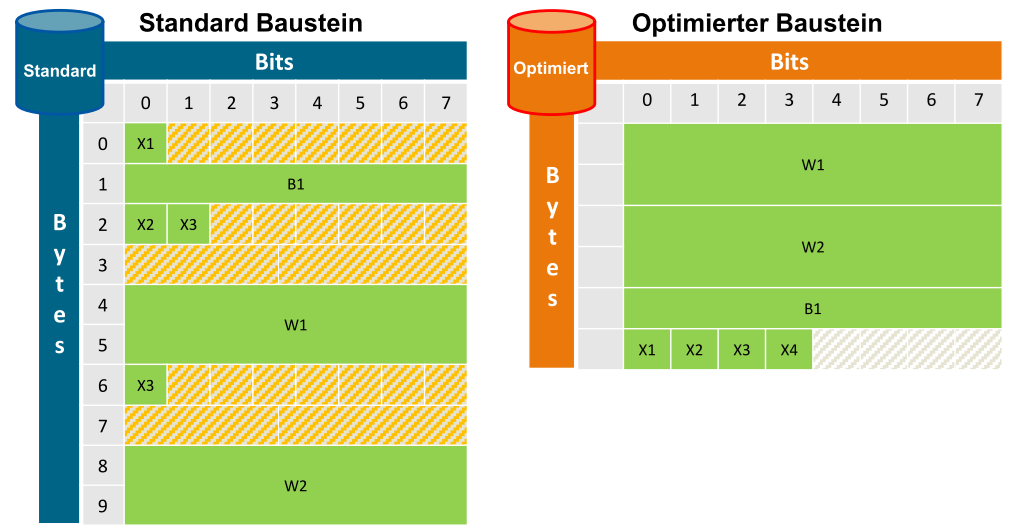
\includegraphics[width = 0.8 \textwidth]{Optimierte_Bausteine_bei_S7-1200.png}
    \caption{Optimierte Bausteine bei S7-1200}
    \label{fig:Optimierte Bausteine bei S7-1200}
\end{figure}

\textbf{Eigenschaften:}\par\noindent
\begin{itemize}
    \item Es entstehen keine Datenlücken, da größere Variablen am Anfang des Bausteins und kleinere am Ende stehen.
    \item Es gibt ausschließlich den symbolischen Zugriff bei optimierten Bausteinen.   
\end{itemize}

\clearpage
\subsection{S7-1500: Aufbau von optimierten Bausteinen}\label{subsec:S7-1500: Aufbau von optimierten Bausteinen}

\begin{figure}[!ht]
    \centering
    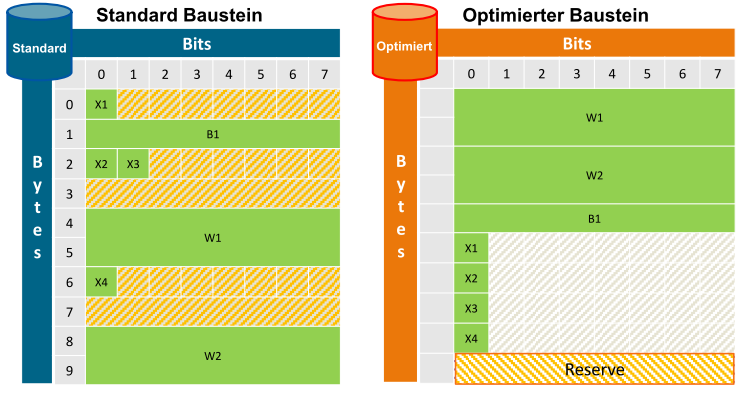
\includegraphics[width = 0.8 \textwidth]{Optimierte Bausteine bei S7-1500.png}
    \caption{Optimierte Bausteine bei S7-1500}
    \label{fig:Optimierte Bausteine bei S7-1500}
\end{figure}
\begin{figure}[!ht]
    \centering
    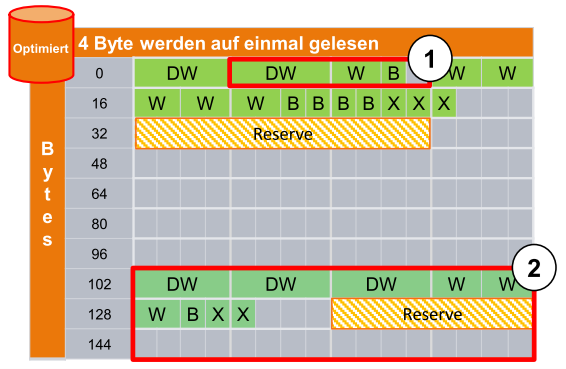
\includegraphics[width = 0.5 \textwidth]{Speicherbelegung bei optimierten Bausteinen.png}
    \caption{Speicherbelegung bei optimierten Bausteinen}
    \label{fig:Speicherbelegung bei optimierten Bausteinen}
\end{figure}

Zu \cref{fig:Speicherbelegung bei optimierten Bausteinen}: \par \noindent
\begin{itemize}
    \item Strukturen liegen separat und können damit als Block kopiert werden.
    \item Remanente Daten liegen in einem separaten Bereich und können als Block kopiert werden. Bei Spannungsausfall werden diese Daten CPU-intern gespeichert. „MRES“ setzt diese Daten auf die im Ladespeicher liegenden Startwerte zurück.
     Bausteinen.   
\end{itemize}

\textbf{Eigenschaften:}\par\noindent
\begin{itemize}
    \item Es entstehen keine Datenlücken, da größere Variablen am Anfang des Bausteins und kleinere am Ende stehen.
    \item Schnellerer Zugriff durch prozessoroptimale Ablage (Alle Variablen werden so abgelegt, dass der Prozessor der S7-1500 sie mit nur einem Maschinenbefehl direkt lesen oder schreiben kann).
    \item Boolesche Variablen werden zum schnellen Zugriff als Byte abgelegt. Somit muss die Steuerung den Zugriff nicht maskieren.
    Bausteinen.   
    \item Optimierte Bausteine haben eine Speicherreserve zum Nachladen im laufenden Betrieb (Siehe Kapitel 6.2.11 Laden ohne Reinitialisierung).
    \item Es gibt ausschließlich den symbolischen Zugriff bei optimierten Bausteinen.
\end{itemize}


\subsection{Prozessoroptimale Datenablage bei S7-1500}\label{subsec:Prozessoroptimale Datenablage bei S7-1500}
Aus Kompatibilitätsgründen zu den ersten SIMATIC Steuerungen wurde das Prinzip der Datenablage „Big-Endian“ in den S7-300/400 Steuerungen übernommen. 
Die neue Steuerungsgeneration S7-1500 greift aufgrund der geänderten Prozessorarchitektur immer auf 4 Byte (32 Bit) in „Little-Endian“-Reihenfolge zu. Dadurch ergeben sich folgende systemseitige Eigenschaften.

\begin{figure}[!ht]
    \centering
    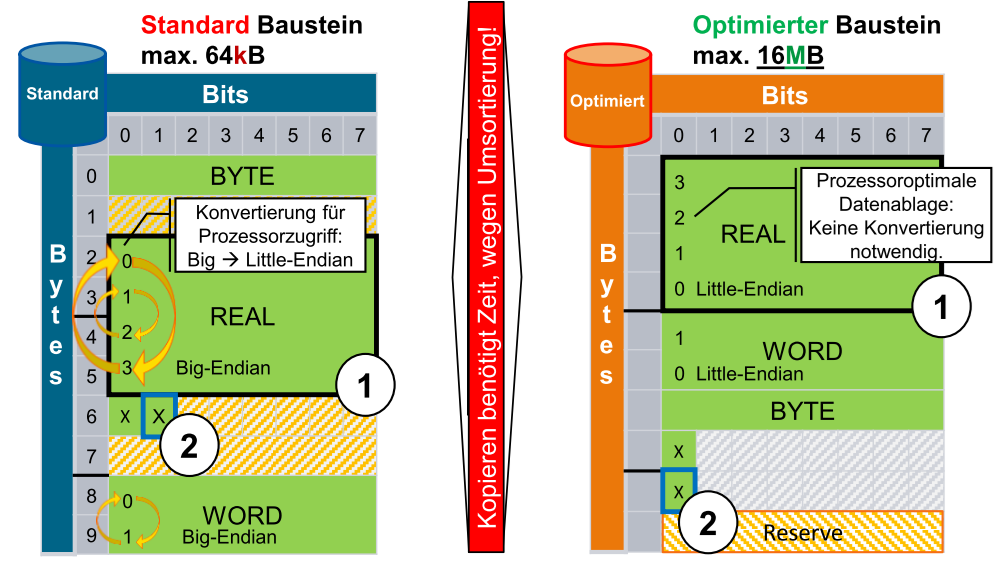
\includegraphics[width = 0.5 \textwidth]{Datenzugriff einer S7-1500 Steuerung.png}
    \caption{Datenzugriff einer S7-1500 Steuerung}
    \label{fig:Datenzugriff einer S7-1500 Steuerung}
\end{figure}

\begin{longtable}{| p{\colwidth{0.06}} | p{\colwidth{0.42}} | p{\colwidth{0.42}} | } % columns widths have to add up to 1 otherwise there will be an over- or underfill of the table layout
    \hline
     & \textbf{Standard Baustein} & \textbf{Optimierter Baustein}  \\    
    \hline
    1. & Bei ungünstigem Offset benötigt die Steuerung  2x16 Bit-Zugriffe, um einen 4-Bytewert (z.B. REAL-Wert) zu lesen. Zusätzlich müssen die Bytes gedreht werden. & Die Steuerung legt die Variablen zugriffsoptimiert ab. Ein Zugriff erfolgt mit 32 Bit (REAL). Eine Drehung der Bytes ist nicht notwendig.  \\    
    \hline
    2. & Pro Bitzugriff wird das komplette Byte gelesen und maskiert. Das komplette Byte wird für jeden anderen Zugriff gesperrt. & Jedes Bit belegt ein Byte. Die Steuerung muss beim Zugriff das Byte nicht maskieren.\\
    \hline
    3. & Maximale Bausteingröße beträgt 64kB. & Maximale Bausteingröße, kann bis zu 16MB betragen.\\
    \hline
    \caption{Datenzugriff einer S7-1500 Steuerung}\label{tab:Datenzugriff einer S7-1500 Steuerung} %\label used for referencing the figure in text
\end{longtable}

\clearpage
\textbf{Empfehlung:}\par \noindent
\begin{itemize}
    \item Verwenden Sie generell nur optimierte Bausteine. 
    \item Sie benötigen keine absolute Adressierung und können immer mit symbolischen Daten (objektbezogen) adressieren. Indirekte Adressierung ist auch mit symbolischen Daten möglich (siehe Kapitel 3.6.2 \textbf{"todo!"}  Datentyp ARRAY und indirekte Feldzugriffe).
    \item Die Abarbeitung von optimierten Bausteinen in der Steuerung ist wesentlich schneller als bei Standardbausteinen. 
    \item Vermeiden Sie das Kopieren/Zuweisen von Daten zwischen optimierten und nicht optimierten Bausteinen. Die dafür erforderliche Umwandlung der Daten zwischen Quell- und Zielformat benötigt eine hohe Abarbeitungszeit.
    
\end{itemize}

\subsection{Weitere Unterschiede}\label{subsec:Weitere Unterschiede}
\begin{longtable}{| p{\colwidth{0.5}} | p{\colwidth{0.5}} | } % columns widths have to add up to 1 otherwise there will be an over- or underfill of the table layout
    \hline
    \textbf{Optimierter Baustein} & \textbf{Nicht optimierter Baustein}  \\    
    \hline
    Optimierte Datenbausteine werden symbolisch adressiert. Deshalb wird kein „Offset“ angezeigt. & Bei nicht optimierten Bausteinen wird der „Offset“ angezeigt und kann zur Adressierung genutzt werden.  \\    
    \hline
    In optimierten Baustein können Sie jede Variable einzeln mit „Remanenz“ (“Retain“) deklarieren. & Im nichtoptimierten Baustein können nur alle oder keine Variable mit „Remanenz“ (“Retain“) deklariert werden.\\
    \hline
    \caption{Unterschied optimierter und nicht optimierter Datenbausteine}\label{tab:Unterschied optimierter und nicht optimierter Datenbausteine} %\label used for referencing the figure in text
\end{longtable}
\noindent Die Remanenz von Variablen eines Global-DB definieren Sie direkt im Global-DB. Standardmäßig ist Nichtremanenz voreingestellt.\par \noindent
Die Remanenz von Variablen einer Instanz definieren Sie im Funktionsbaustein (nicht im In-stanz-DB). Diese Einstellungen gelten damit für alle Instanzen dieses FBs.

\clearpage
\subsection{Zugriffsarten bei optimierten und nicht optimierten Bausteinen}\label{subsec:Zugriffsarten bei optimierten und nicht optimierten Bausteinen
}
\begin{longtable}{| p{\colwidth{0.33}} | p{\colwidth{0.33}} | p{\colwidth{0.33}} |} % columns widths have to add up to 1 otherwise there will be an over- or underfill of the table layout
    \hline
    \textbf{Zugriffsart} & \textbf{Optimierter Baustein} & \textbf{Nicht optimierter Baustein} \\    
    \hline
    Symbolisch & Ja & Ja\\    
    \hline
    Indizierte (Felder) & Ja & Ja\\
    \hline
    Slice - Zugriffe & Ja & Ja\\
    \hline
    AT-Anweisung & Nein (Alternative: Slice-Zugriff) & Ja\\
    \hline
    Direkt Absolut & Nein (Alternative: Array mit Index) & Ja\\
    \hline
    Direkt Absolut (Zeiger)& Nein (Alternative: VARIANT / Array mit Index) & Ja\\
    \hline
    Laden ohne Reinitialisierung& Ja & Nein\\
    \hline
    \caption{Zugriffsarten}\label{tab:Zugriffsarten} %\label used for referencing the figure in text
\end{longtable}

\noindent \textbf{Hinweis:}\par \noindent
Weitere Informationen finden Sie in folgenden Beiträgen:
Welche Unterschiede müssen Sie zwischen der optimierten Datenablage und dem Standard-Bausteinzugriff in STEP 7 (TIA Portal) beachten? \\
\url{https://support.industry.siemens.com/cs/ww/de/view/67655611}
\noindent 
Welche Eigenschaften müssen Sie in STEP 7 (TIA Portal) bei den Anweisungen 
\glqq READ\_DBL\grqq{} und \glqq WRIT\_DBL\grqq{} beachten, wenn Sie DBs mit optimiertem Zugriff verwenden? \\
\url{https://support.industry.siemens.com/cs/ww/de/view/51434747}


\subsection{Konvertierung zwischen optimierten und nicht optimierten Variablen}\label{subsec:Konvertierung zwischen optimierten und nicht optimierten Variablen}
Grundsätzlich wird empfohlen mit optimierten Variablen zu arbeiten. Falls man aber in Einzelfällen seine bisherige Programmierung beibehalten möchte, ergibt sich eine Mischung von optimierter und nicht optimierter Datenablage im Programm. \par
Das System kennt die interne Ablage jeder Variablen, egal ob strukturiert (von einem selbst definierten Datentyp abgeleitet) oder elementar (INT, LREAL, …).\par 
Bei typgleichen Zuweisungen zwischen zwei Variablen mit unterschiedlicher Speicherablage konvertiert das System automatisch. Diese Konvertierung benötigt bei strukturierten Variablen Performance und sollte deshalb möglichst vermieden werden.

\subsection{Parameterübergabe zwischen Bausteinen mit optimiertem und nicht optimierten Zugriff}\label{subsec:Parameterübergabe zwischen Bausteinen mit optimiertem und nicht optimierten Zugriff}

Wenn bei einem Bausteinaufruf Strukturen als Durchgangsparameter (InOut) an den aufgeru-fenen Baustein übergeben werden, werden diese standardmäßig als Referenz übergeben (siehe Kapitel 3.3.2 \textbf{"todo!"} Übergabe per Referenz (Call-by-reference) mit InOut-Schnittstellentyp). \par
Dies gilt jedoch nicht, wenn einer der Bausteine die Eigenschaft \glqq Optimierter Zugriff\grqq{} und der andere Baustein die Eigenschaft \glqq Standardzugriff\grqq{} hat. Dann werden grundsätzlich alle Parameter als Kopie übergeben (siehe Kapitel 3.3.1 \textbf{"todo!"} Übergabe per Wert (Call-by-value) mit In-Schnittstellentyp). \par
Der aufgerufene Baustein arbeitet in diesem Fall immer mit den kopierten Werten. Während der Bausteinbearbeitung werden diese Werte möglicherweise verändert und nach Abarbeitung des Bausteinaufrufs wieder auf den ursprünglichen Operanden zurückkopiert. \par
Dies kann zu Problemen führen, wenn die ursprünglichen Operanden durch asynchrone Prozesse verändert werden, z.B. durch HMI-Zugriffe oder durch Alarm-OBs. Wenn nach der Bausteinbearbeitung die Kopien wieder auf die ursprünglichen Operanden zurückkopiert werden, werden dabei die asynchron durchgeführten Änderungen an den ursprünglichen Operanden überschrieben.

\noindent \textbf{Hinweis:}\par \noindent
Weitere Informationen finden Sie in folgenden Beitrag: 
Warum kann es zum Überschreiben von Daten des HMI-Systems oder des Webservers in der S7-1500 kommen? 
\url{https://support.industry.siemens.com/cs/ww/de/view/109478253}

\noindent \textbf{Empfehlung:}\par \noindent
Stellen Sie immer in beiden Bausteinen, die miteinander kommunizieren dieselbe Zugriffsart ein.

\subsection{Kommunikation mit optimierten Daten}\label{subsec:Kommunikation mit optimierten Daten}
Die Schnittstelle (CPU, CM) überträgt die Daten so, wie sie angeordnet sind (unabhängig ob optimiert oder nicht optimiert).


\begin{figure}[!ht]
    \centering
    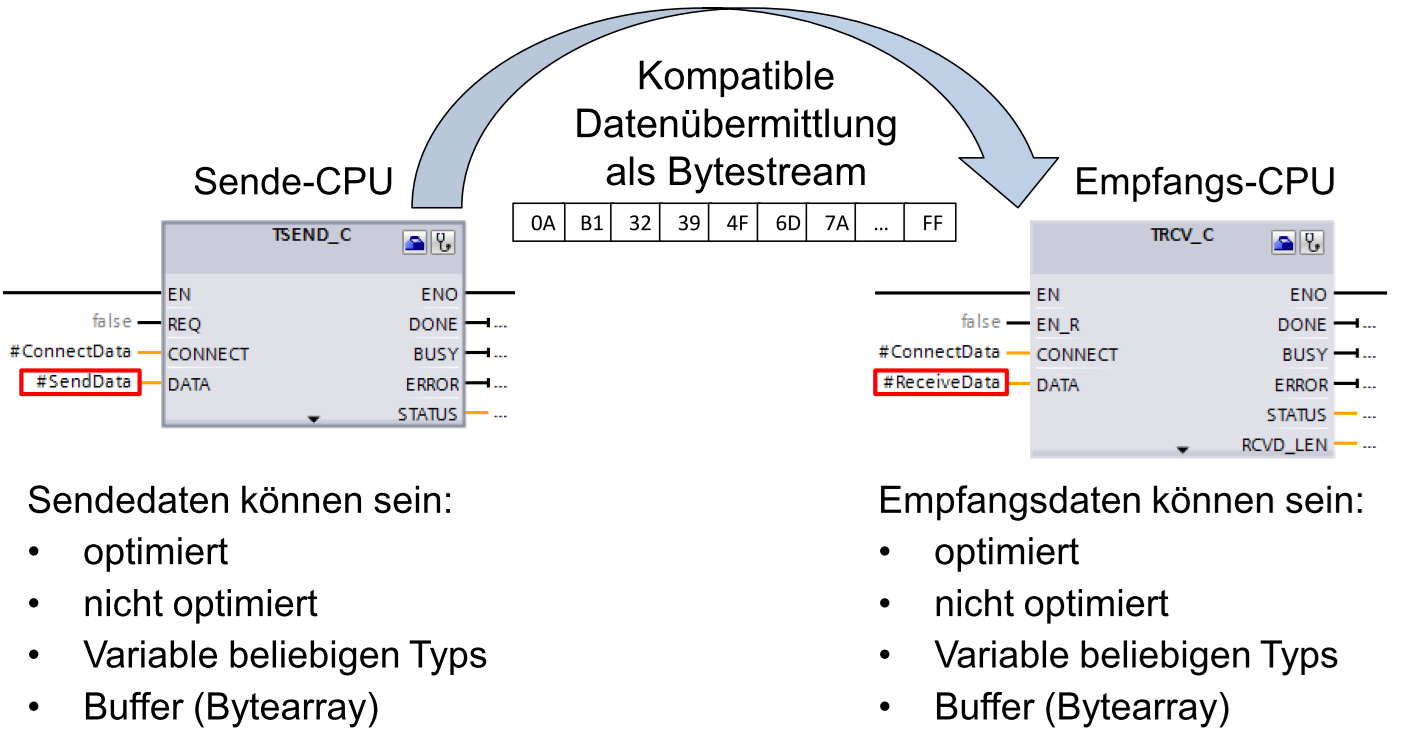
\includegraphics[width = 0.5 \textwidth]{CPU-CPU Kommunikation.png}
    \caption{CPU-CPU Kommunikation}
    \label{fig:CPU-CPU Kommunikation}
\end{figure}